\documentclass[12pt]{article}
\usepackage[french]{babel}
\usepackage[utf8x]{inputenc}
\usepackage{amsmath}
\usepackage{graphicx}
\usepackage[colorinlistoftodos]{todonotes}
\usepackage{float}
\usepackage{graphicx}
\usepackage{caption}
\usepackage{subcaption}
\usepackage{adjustbox}
\usepackage[euler]{textgreek}
\usepackage[left=1in,right=1in,top=1in,bottom=1in]{geometry}
%\usepackage{subfigure}
\usepackage{comment}
\usepackage{caption}
\usepackage{lastpage}
\usepackage[colorlinks,pdfpagelabels,pdfstartview = FitH,bookmarksopen = true,bookmarksnumbered = true,linkcolor = black,plainpages = false,hypertexnames = true,citecolor = black,pagebackref = true,urlcolor = black] {hyperref}
\usepackage{setspace}
\usepackage{silence}
\WarningFilter{latex}{Text page}
\usepackage{parskip}
\newcommand{\cms}{~cm\textsuperscript{-2}s\textsuperscript{-1} }

\graphicspath{{figures/}}   
% \renewcommand{\figurename}{Fig.}
\addto\captionsenglish{\renewcommand{\figurename}{Fig.}}

\begin{document}

\begin{titlepage}

\newcommand{\HRule}{\rule{\linewidth}{0.5mm}} % Defines a new command for the horizontal lines, change thickness here

\center % Center everything on the page
 
%----------------------------------------------------------------------------------------
%	HEADING SECTIONS
%----------------------------------------------------------------------------------------

\textsc{\LARGE Universit\'e Claude Bernard Lyon I}\\[1.5cm] % Name of your university/college
\textsc{\Large Master Data Science}\\[0.5cm] % Major heading such as course name
\textsc{\large Mod\`eles de r\'egression}\\[0.5cm] % Minor heading such as course title

%----------------------------------------------------------------------------------------
%	TITLE SECTION
%----------------------------------------------------------------------------------------

\HRule \\[0.4cm]
{ \huge \bfseries R\'egression des donn\'ees d'extraction de puits de p\'etrole au Canada}\\[0.4cm] % Title of your document
\HRule \\[1.5cm]
 
%----------------------------------------------------------------------------------------
%	AUTHOR SECTION
%----------------------------------------------------------------------------------------

\begin{minipage}{0.4\textwidth}
\begin{flushleft} \large
\emph{Auteurs:}\\
Bruno \textsc{Dumas}\\% Your name
Jules \textsc{Sauvinet}
\end{flushleft}
\end{minipage}
~
\begin{minipage}{0.4\textwidth}
\begin{flushright} \large
\emph{Professeur:} \\
Fran\c cois \textsc{Wahl} % Supervisor's Name
\end{flushright}
\end{minipage}\\[2cm]

% If you don't want a supervisor, uncomment the two lines below and remove the section above
%\Large \emph{Author:}\\
%John \textsc{Smith}\\[3cm] % Your name

%----------------------------------------------------------------------------------------
%	DATE SECTION
%----------------------------------------------------------------------------------------

{\large \today}\\[1cm] % Date, change the \today to a set date if you want to be precise

%----------------------------------------------------------------------------------------
%	LOGO SECTION
%----------------------------------------------------------------------------------------


\includegraphics[height=5cm]{ucbl}\\[1cm] % Include a department/university logo - this will require the graphicx package
 
%----------------------------------------------------------------------------------------

\vfill % Fill the rest of the page with whitespace

\end{titlepage}

\begin{abstract}
L'objectif est d'effectuer des r\'egressions des valeurs d'extractions des puits de p\'etrole du Canada afin de pouvoir pr\'edire les future donn\'ees d'extraction. 
Les courbes des valeurs des donn\'ees d'extraction donne une classification de la qualit\'e des puits.
L'objectif de ce travail est de mettre en place une classification automatique de ces puits: La
d\'emarche propos\'ee est d\'ecrite ci-dessous.
L'id\'ee est de remplacer ces courbes par des fonctions param\'etriques.
Pour cela, plusieurs r \'egressions vont \^etre envisag\'ees afin d'avoir la meilleure pr\'ediction/classification possible.
\end{abstract}

%\begin{spacing}{1.15}
\pdfbookmark[1]{Contents}{toc}
\small{
\tableofcontents 
}
\newpage
% \listoffigures
% \newpage
% \listoftables 
%\end{spacing}


\section{R\'egressions polynomiales}
\label{sec:reg_pol}

Une fa\c con simple est d'ajuster un polyn\^ome de degr\'e faible sur chacune des courbes et
de voir si les coefficients pr\'esentent des clusters, c'est \`a dire des groupes de points distincts
quand on les regarde dans l'espace.
On essaiera des polyn\^omes de degr\'e 0, 1, 2, 3, et 4.
On pr\'esentera les courbes de production simul\'ees obtenues, comme dans la figure ci-dessous.

%\figurename~\ref{fig:sspc_mpc} shows a basic laboratory setup for SSPC. The temperature of the probe is controlled with a cryostat. A voltage is applied to the probe and the current is measured with an electrometer under illumination produced with LEDs. A neutral filter can be used to further reduce the intensity of the light. The intensity of the LEDs could also be modulated and the current be measured with a lock-in amplifier (this will be covered in section~\ref{sec:mpc}).
%This is shown in figure \ref{fig:cutoff_example}.
 
\begin{figure}[H]
 \centering % avoid the use of \begin{center}...\end{center} and use \centering instead (more compact)
	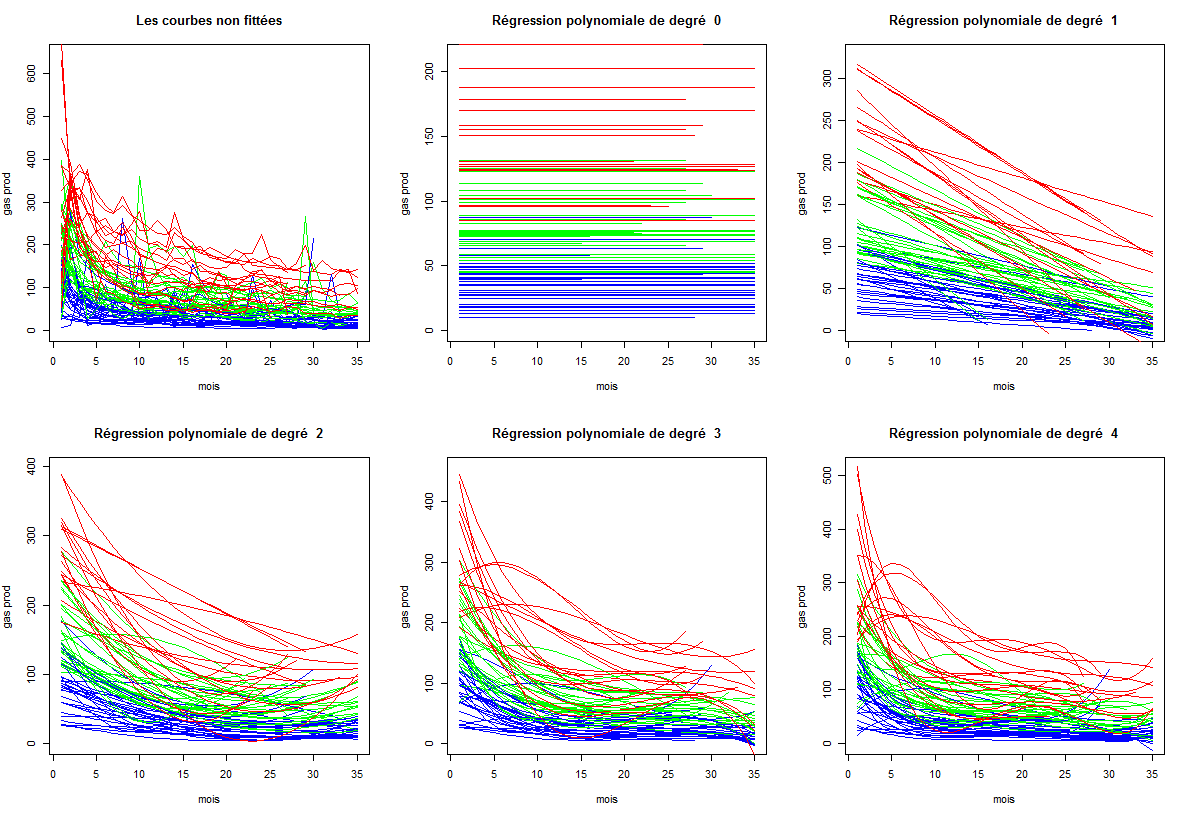
\includegraphics[width=250px]{reg_pol}
  \caption{\label{fig:polynomial_regressions} Courbes non r\'egress\'ees, et courbes de r\'egressions polynomiales de degr\'es $0$,$1$,$2$,$3$ et $4$}
\end{figure}

La moyenne des R-Squared ajusted pour les $75$ courbes pour les $5$ types de r\'egression sont respectivement : 
\newline
$0.0000000$, $0.4853609$, $0.6622269$, $0.7202006$ et $0.7557633$.
\newline
On voit que plus le degr\'e du polynome augmente, plus la r\'egression est de qualit\'e au cri\`ere du R-Squared (les valeurs pr\'edites se rapprochent des valeurs des observations.

Si on se r\'ef\`ere \`a la figure ci-dessus, on observe que la plupart des simulations
pr\'esente une remont\'ee au bout de quelques mois, que certaines simulations sont concaves
au lieu d'\^etre convexes, voire que certaines d'entre elles pourraient avoir des valeurs n\'egatives (autour des $35$ mois d'exploitation).

\newpage


\section{R\'egressions exponentielles}

Une id\'ee simple pour corriger ces d\'efauts est d'utiliser une autre forme param\'etrique pour
les simulations. Une suggestion imm\'ediate pour qui a un peu l'habitude de ces courbes est
une forme exponentielle du style : o\'u $y$ est la production, $t$ le mois, et $k0$ et
$k1$ deux param\`etres \'a d\'eterminer.

\textbf{R\'egression exponentielle avec lm}

\begin{figure}[H]
 \centering % avoid the use of \begin{center}...\end{center} and use \centering instead (more compact)
	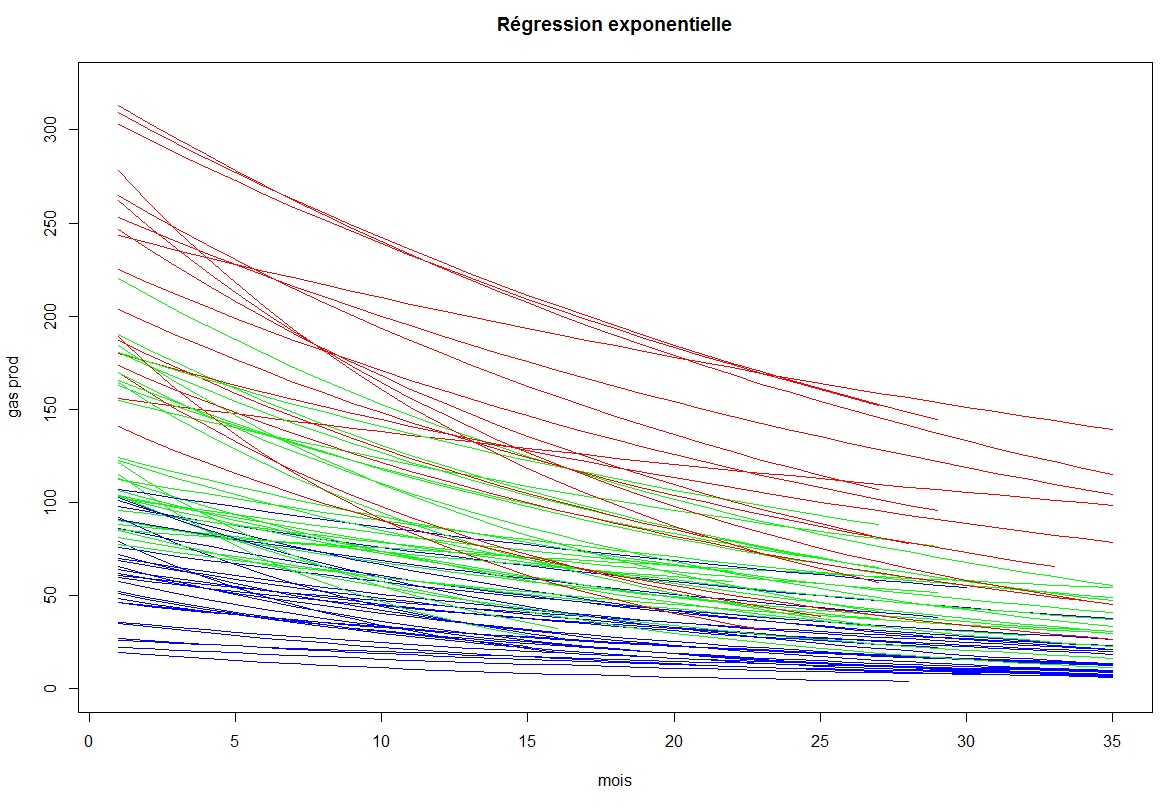
\includegraphics[width=250px]{reg_exp_1}
  \caption{\label{fig:exponential_reg_lm} Courbes r\'egress\'ees avec une fonction exponentielle et et la fonction lm de R}
\end{figure}


\textbf{R\'egression exponentielle avec nls}

\begin{figure}[H]
 \centering % avoid the use of \begin{center}...\end{center} and use \centering instead (more compact)
	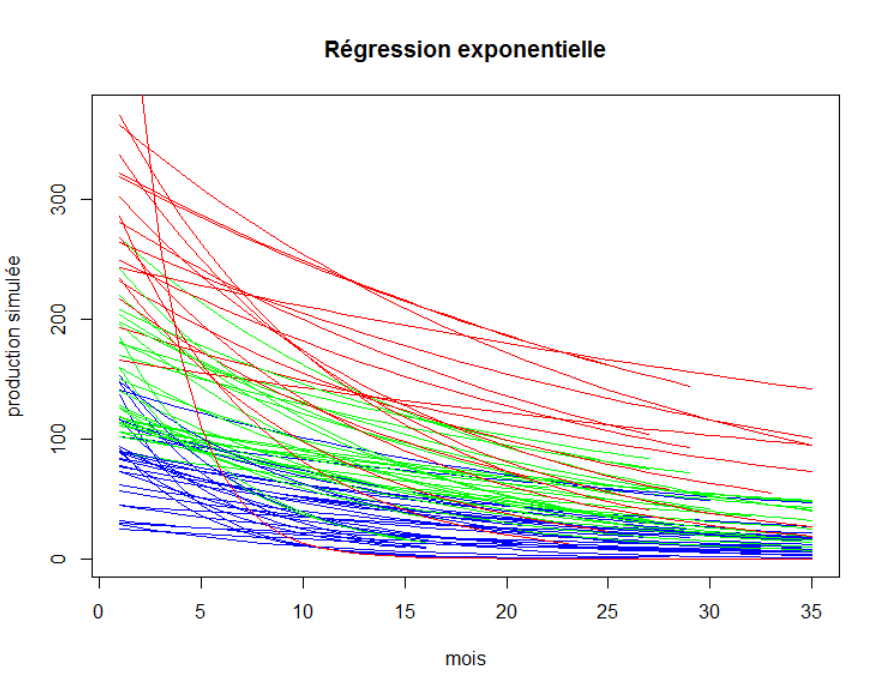
\includegraphics[width=250px]{reg_exp_2}
  \caption{\label{fig:exponential_reg_nls} Courbes r\'egress\'ees avec une fonction exponentielle et et la fonction nls de R}
\end{figure}


La r\'egression avec lm para\^it mieux, on s'int\'eressera donc \'a celle-ci.

Est-ce que cela marche ? 
La moyenne du "ajusted R-Squared" pour les 75 r\'egressions exponentielles est cette fois-ci de $0.6754964$, donc de moins bonne quali\'e \'a priori que les r\'egressions polynomiales de degr\'e sup\'erieures ou \'egale \'a $3$. N\'eanmoins, quand on s'int\'eresse au d\'etail des R-Squared, on trouve de tr\'es bonne r\'egressions avec un R-Squared tr\`es bon comme des r\'egressions avec un R-Squared tr\`es mauvais. Cela est probablement d\^u à certaines valeurs "outliers" qui ne permettent pas \'a la fonction exponentielle de s'adapter aux courbes. La partie $5$ et le lissage des courbes permettra de pallier \'a ce probl\`eme et de probablement monter que la r\'egression exponentielle est adapt\'ee si un travail d'att\'enuation des "pics" est fait au pr\'ealable.
$10$ premiers R-Squared : $0.8011383$, $0.4182548$, $0.7403922$, $0.7585257$, $0.4186529$, $0.6888943$, $0.3297291$, $0.818889$, $0.7745934$
et $0.7527809$.

Avez-vous d'autres id\'ees ?
R\'egression avec fonction inverse, ou gaussienne? 
\newline
Ou bien une composé de polyn\^ome dans un logarithme.

\newpage

\section{Courbes hautes et basses \'a 95\%}

Quelles sont les incertitudes sur les r\'egressions des points 2 ? Plus concr\`etement, on
vous demande de tracer pour un exemple de chaque type de courbe, la courbe haute (\'a
95\%) et la courbe basse (toujours \'a 95\%)

\textbf{Intervalles de confiance}

\begin{figure}[H]
 \centering % avoid the use of \begin{center}...\end{center} and use \centering instead (more compact)
	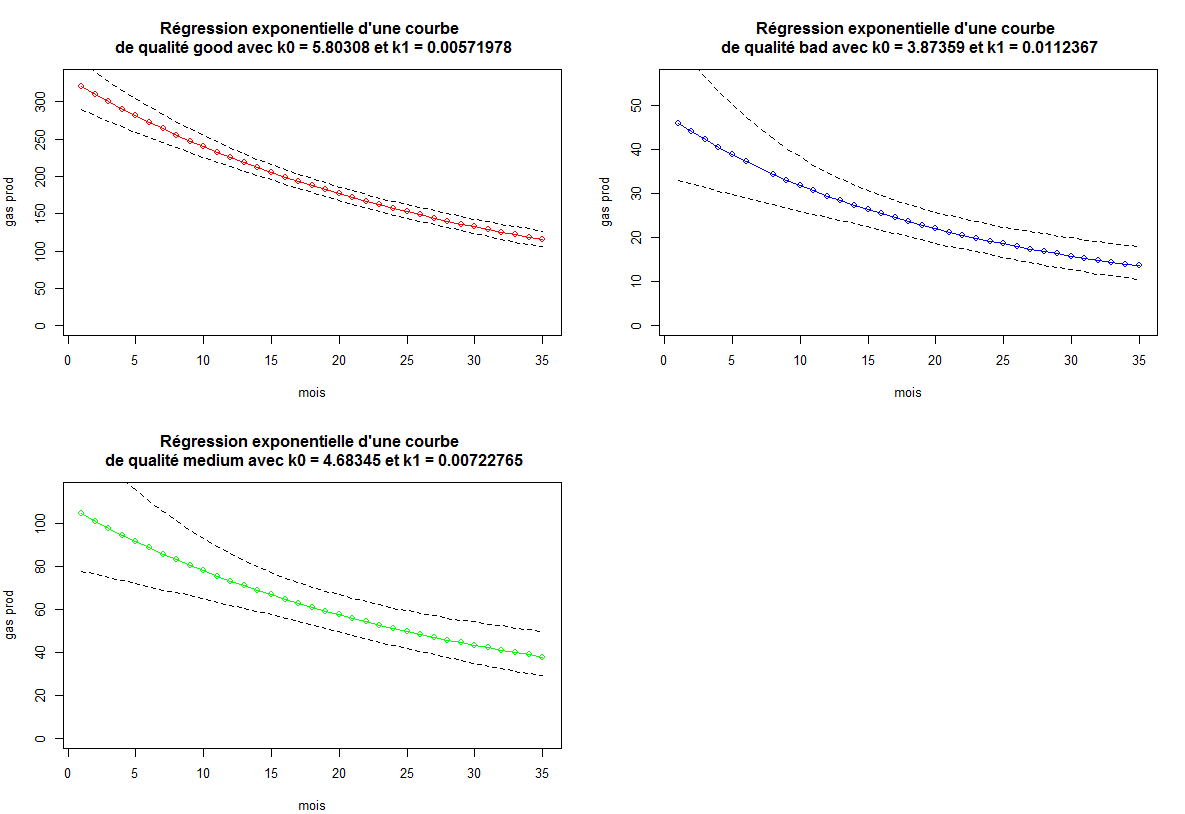
\includegraphics[width=400px]{q3_predict_nls}
  \caption{\label{fig:q3_predict_nls} Courbes hautes et basses à 95\% pour un exemple de chaque classes de courbes}
\end{figure}


\textbf{Avec bootstraping}

%\begin{figure}[H]
% \centering % avoid the use of \begin{center}...\end{center} and use \centering instead (more compact)
%	\includegraphics[width=250px]{q3_bootstrap}
%  \caption{\label{fig:q3_predict_nls} Courbes hautes et basses pour un exemple de 3 classes de courbes}
%\end{figure}

\newpage
\section{Reclassement avec r\'egression logistique}
 
En examinant le graphe k1 fonction de k0, on se rend compte que certaines courbes
class\'ees 'Good' par les experts donnent l'impression d'\^etre plut\^ot 'medium', tandis que
certaines 'bad' pourraient \^etre aussi 'medium'. 
\newline
Avez-vous des suggestions sur 5 courbes au
plus qui pourraient \^etre mal class\'ees ? Justifiez vos choix (i.e. une fa\c con de faire est
d'effectuer une r\'egression logistique dont le y est la classe pr\'edite par l'expert et les x sont
les coefficients k0 et k1, et d'examiner comment la r\'egression est am\'elior\'ee en changeant la
classe d'un point ; une autre fa\c con plus empirique est de d\'eterminer deux droites x=k11 et
x=k12 qui partitionnent au mieux les classes et d'examiner comme pr\'ec\'edemment comment
la classification est chang\'ee en basculant certains points d'une classe \'a l'autre).

\textbf{$k1$ en fonction de $k0$}

\begin{figure}[H]
 \centering % avoid the use of \begin{center}...\end{center} and use \centering instead (more compact)
	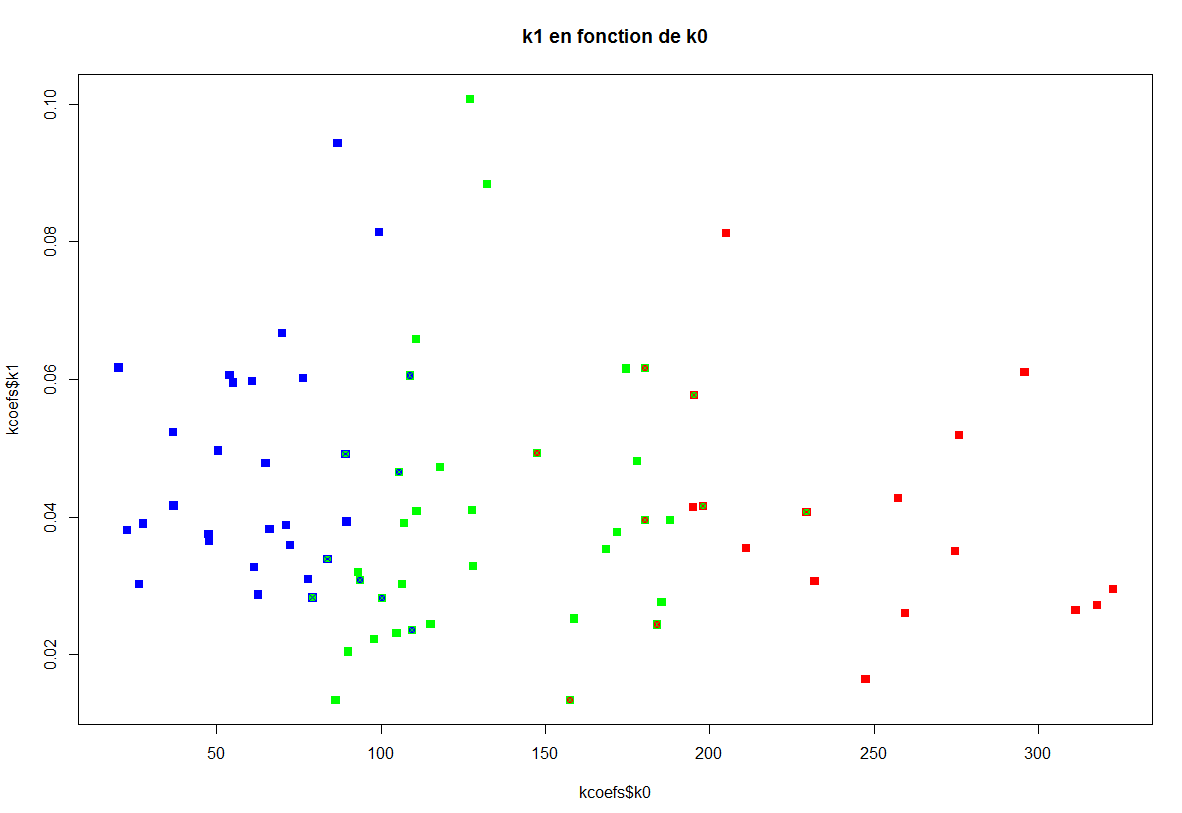
\includegraphics[width=250px]{clustering}
  \caption{\label{fig:k0_k1} Coefficients $k1$ en fonction de $k0$}
\end{figure}

TODO explain
TODO changer de classe etc.


\newpage

\section{Gestion des spikes et lissage des courbes}

\textbf{R\'egression polynomiale de degr\'e 3 avec lissage loess}

\begin{figure}[H]
 \centering % avoid the use of \begin{center}...\end{center} and use \centering instead (more compact)
	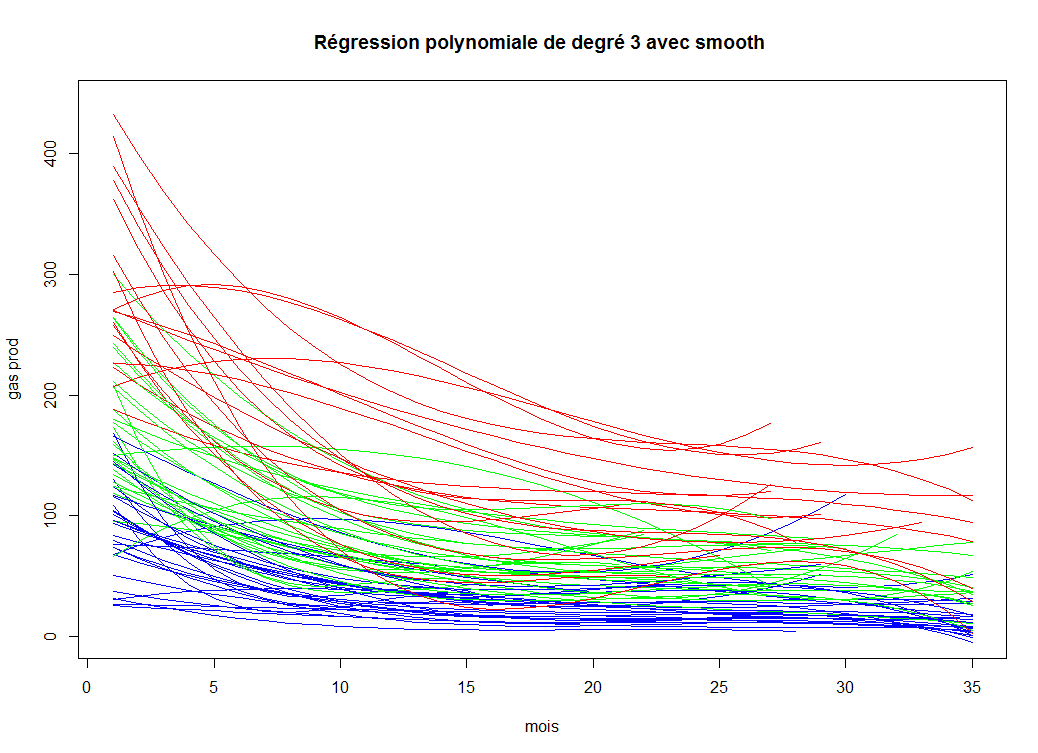
\includegraphics[width=250px]{reg_pol3_smooth_loess}
  \caption{\label{fig:reg_pol3_smooth_loess} R\'egression polynomiale de degr\'e 3 avec courbes liss\'ee au pr\'ealable avec loess}
\end{figure}

On obtient une moyenne de R-Squared de $0.9802724$ cette fois-ci apr\`es lissage des courbes. La r\'egression polynomiale devient ainsi tr\`es performante. Il reste \`a savoir si l'on peut se permettre l'approximation fa\^ite par le lissage des courbes et si les valeurs induites par les spikes avait une pertinence intransigible. Toutefois, la r\'egression avec smooth ne r\`egle pas les valeurs qui remontent, les simulations concaves au lieu d'\^etre convexes, et les potentielles valeurs n\'egatives autour des $35$ mois.

\textbf{R\'egression exponentielle avec lissage loess}

\begin{figure}[H]
 \centering % avoid the use of \begin{center}...\end{center} and use \centering instead (more compact)
	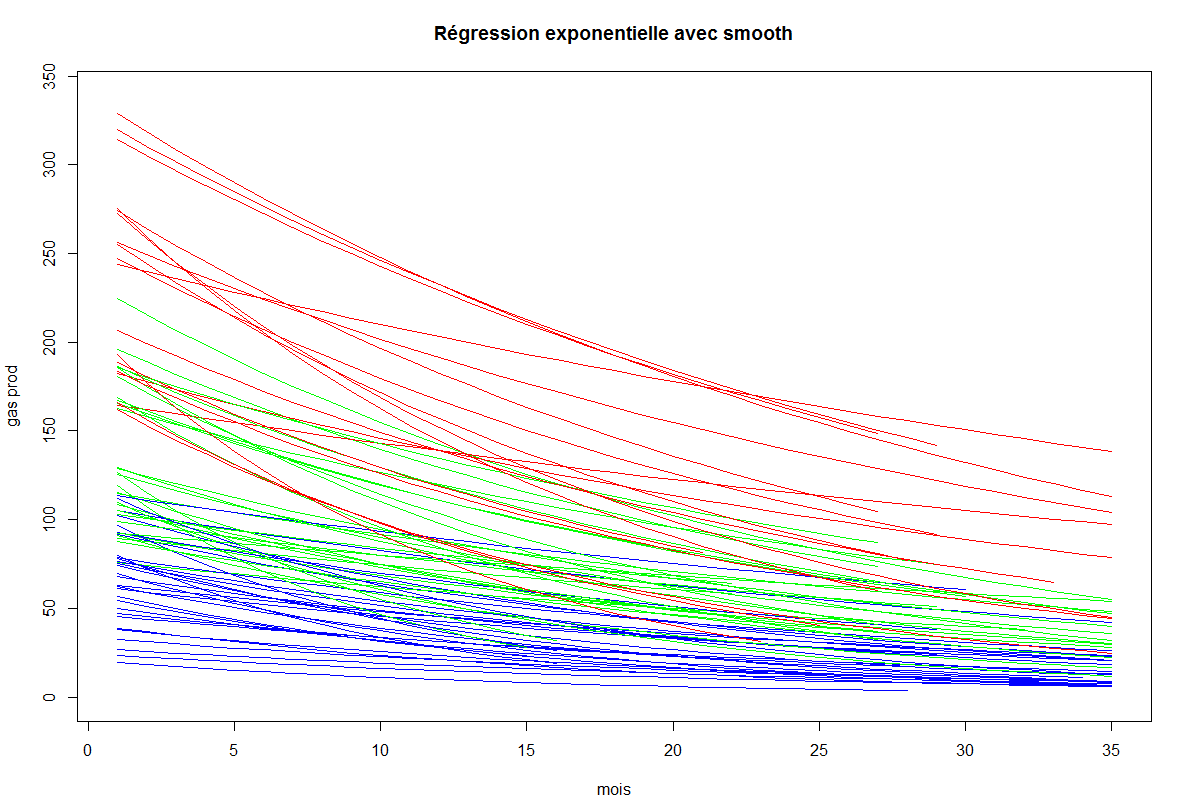
\includegraphics[width=250px]{reg_exp_smooth_loess}
  \caption{\label{fig:reg_exp_smooth_loess} R\'egression exponentielle lm avec courbes liss\'ee au pr\'ealable avec loess}
\end{figure}

On obtient une moyenne de R-Squared de $0.845492$ cette fois-ci apr\`es lissage des courbes. La r\'egression est sensiblement am\'elior\'ee avec le lissage des courbes mais reste moins efficace que la r\'egression polynomiale de degr\'e 3.

\newpage

\section{Conclusion}

TODO TOO


\section*{Acknowledgments}
Merci \'a Fran\c cois Wahl.

\end{document}